\thispagestyle{empty}
\chapter{本研究のアプローチ}
\label{chap2}
\minitoc

\newpage
%%%%%%%%%%%%%%%%%%%%%%%%%%%%%%%%%%%%%%%%%%%%%%%%%%%%%%%%%%%%%%%%%%%%%%%%%%%%%%%
%==============================================================================
% 2.1
%==============================================================================
\section{はじめに}

本章では,本研究のアプローチについて述べる.

まず2.2節にて,本研究における問題設定について述べる.

2.3節にて,本手法の全体像について述べる.

2.4節にて,本手法のアプローチと解決すべき課題について述べる.
2.4.1項にて,姿勢を推定するためのアプローチについて述べる.
2.4.2項にて,位置を推定するためのアプローチについて述べる.


\clearpage
%==============================================================================
% 2.2
%==============================================================================
\section{問題設定}

第1章にて,全天球カメラの高速な6自由度の位置姿勢推定手法が重要であることを述べた.
特に,GPSが利用できない屋内環境で適用できる手法の構築が重要である.
\\

また,1.2節にて,環境のモデルを参照情報として,1枚の画像を用いて環境中から大域的に推定することを述べた.
屋内環境は人工物のため,建設用のCADモデルなどの3次元モデルを容易に入手可能である.
建設用のCADモデルがない場合にも,一度レーザレンジファインダ等で計測すれば,その後は計測したモデルを用いることができる.
従って,本研究では環境の3次元モデルを参照情報として利用する.
\\

適用する主なアプリケーションとしては,屋内環境でドローンを利用する際,位置姿勢推定の初期値を定めることを想定する.
ここで,ドローンの姿勢変化は地面に対して垂直な軸回りの回転が主なものであり,その他の軸回りの回転は微小である.
これにより,推定するカメラ座標系における上下方向の座標軸は,ワールド座標系における上下方向の座標軸の方向に近い方向を持つことが言え,この前提条件を姿勢推定において用いる.
\\

上記を踏まえて,本研究の問題設定を以下にまとめる.
\begin{itemize}
  \item 全天球カメラの6自由度の位置姿勢を推定する.
  \item 1枚の画像を用いて環境中から大域的に推定する.
  \item 3次元モデルが入手可能な屋内環境を対象とする.
  \item 姿勢変化は,地面に対して垂直な軸回りの回転が主である.
\end{itemize}

このような問題設定の下,全天球カメラの高速な位置姿勢推定手法を提案する.

\clearpage
%==============================================================================
% 2.3
%==============================================================================
\section{本手法の全体像}

2.2節で述べた通り,参照情報として環境の3次元モデルを用いる.
本研究では,屋内環境を対象とするため,壁と床の交線など,直線が多数存在することから,直線情報を用いる.
%直線は一部が隠れた場合でも,見えている部分から直線検出が可能であるため,人などの移動物体による遮蔽に対してもロバストであるというメリットがある.
直線情報は構造物の形状を反映したものであるため,環境の3次元モデルにおいては色情報がないモデルにおいても適用可能となる.
従って,本研究では直線情報を用いた高速な位置姿勢推定手法を提案する.
\\

提案手法の全体の流れを図\ref{fig:flow2}に示す.
はじめに,全天球カメラ画像から直線の方向に関する情報を含む直線特徴を抽出し,1枚の全天球カメラ画像のみからカメラの姿勢を推定する.
続いて,推定された姿勢をもとに,直線の位置に関する情報を含む直線特徴を抽出し,3次元モデルから抽出した直線特徴と比較することにより,カメラの位置を推定する.
全天球カメラ画像からは,エッジ点における勾配を利用することで直線特徴を抽出する.
環境の3次元モデルからは,事前にモデルをラインマップに変換しておくことで,ラインマップから直接直線特徴を抽出する.
このように,姿勢と位置を分離して推定することにより,探索空間の次元を削減することができ,局所解に陥る可能性を減らすことができる.
\\

次節以降で,姿勢推定と位置推定それぞれの具体的なアプローチについて説明する.



\begin{figure}[b]
 \begin{center}
 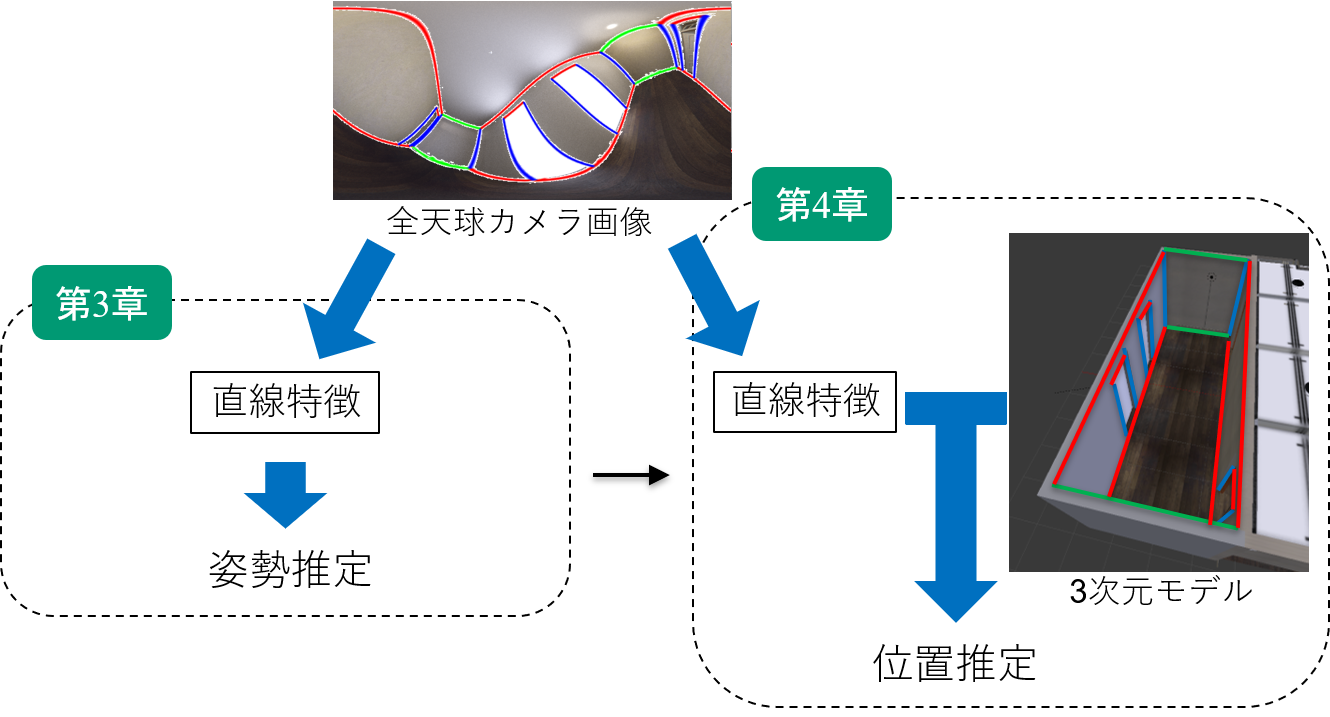
\includegraphics[width=0.9\columnwidth]{./chap2/fig/flow2.png}
 \vspace{5mm}
 \caption{提案手法の全体像}
 \label{fig:flow2}
 \end{center}
\end{figure}


\clearpage
%==============================================================================
% 2.4
%==============================================================================
\section{アプローチ}

\subsection{姿勢推定}

カメラの姿勢は,基準となる位置姿勢からの回転を推定することで推定することができる.
カメラの回転を推定する手法はこれまでにも多く提案されており,2枚の画像間の回転を推定する手法と,1枚の画像を用いてワールド座標系からの回転を推定する手法に分けられる.
前者の手法を用いて姿勢を推定する場合,事前に基準となる位置姿勢で画像を取得しておき,基準となる画像からの回転を推定することで姿勢が得られる.
後者の手法を用いる場合,推定した回転がそのままカメラの姿勢を表す.
\\

2枚の全天球カメラ画像間の回転を推定する手法として,Makadiaらは,画像に球面フーリエ変換を適用し,位相変移を最小化することで回転を推定する手法を提案している\mbox{\cite{Makadia2003}}\mbox{\cite{Makadia2004}}\mbox{\cite{Makadia2006}}.
しかし,この手法は位置が大きく変化して画像の内容が変わってしまうような場合には適用することができない.
また,Kimらは,画像全体におけるオプティカルフローを入力とした学習ベースの回転推定を行っている\mbox{\cite{Kim2019}}.
しかし,画像間の並進量が大きい場合には画像全体におけるオプティカルフローが得られず,回転を推定することができない.
これらの手法のように,画像間の並進量に制限がある回転推定手法を用いて姿勢を推定する場合,事前に取得した基準画像の近くで取得する画像に対してのみしか適用できない.
\\

一方で,1枚の画像を用いてワールド座標系からの回転を推定する手法では,画像を取得する位置に関わらず姿勢を推定することができる.
1枚の画像を用いてワールド座標系からの回転を推定する手法では,消失点が用いられる.
消失点とは,環境中で互いに平行な直線が投影された画像内で交わる点であり,3次元空間では無限遠点に相当するため,カメラの位置変化の影響は無視でき,消失点の位置から姿勢を推定できる.
特に,環境中の直線は互いに直交する3方向のいずれかの方向であるというマンハッタンワールド仮説\mbox{\cite{Coughlan2001}}の下,この3つの主方向の情報から姿勢を推定する手法が多く提案されている.
Kimらは,平面の法線ベクトルを用いて主方向を求める手法を提案している\mbox{\cite{Kim2017}}.
しかし,この手法にはデプスマップが必要となり,1枚の画像のみから姿勢を推定することはできない.
法線ベクトルではなく,画像内で検出された直線を用いて主方向を求める手法も提案されている\mbox{\cite{Bazin2012a}}\mbox{\cite{Elloumi2012}}\mbox{\cite{Elloumi2013}}\mbox{\cite{Lee2015}}.
また,勾配のみから主方向を求める手法も存在する\mbox{\cite{Antone2000}}\mbox{\cite{Martins2005}}\mbox{\cite{Denis2008}}.
勾配のみからの推定では,直線の検出が必要ないため,高速に推定することができる.
しかし,勾配のみから主方向を求めているこれらの手法では通常の透視投影カメラを用いており,全天球カメラの姿勢推定に適用することはできない.
Liらは,全天球カメラ画像のエッジ点における勾配から消失点を推定している\mbox{\cite{Li2012}}.
しかし,この研究では3方向全ての消失点を求めていない.
また,すべてのエッジ点を同様に扱っているが,全天球カメラ画像には歪みが含まれており,歪みの大きな領域のエッジ点における勾配の計算精度が低下することから,回転推定の精度も低下してしまうと考えられる.
\\

以上のことをふまえ,人工物である屋内環境を対象とする本研究では,図\ref{fig:manhattan}に赤,緑,青の線で示すように互いに直交する3方向の直線が多く存在することを利用して,1枚の画像から互いに直交する3方向を求めてワールド座標系からの回転を推定することにより,全天球カメラの姿勢推定を行う.
特に,全天球カメラ画像のエッジ点における勾配のみから高速に3方向を推定する手法を提案する.
また,勾配を計算する際に歪みを考慮することで計算精度を高める.

\begin{figure}[b]
 \begin{center}
 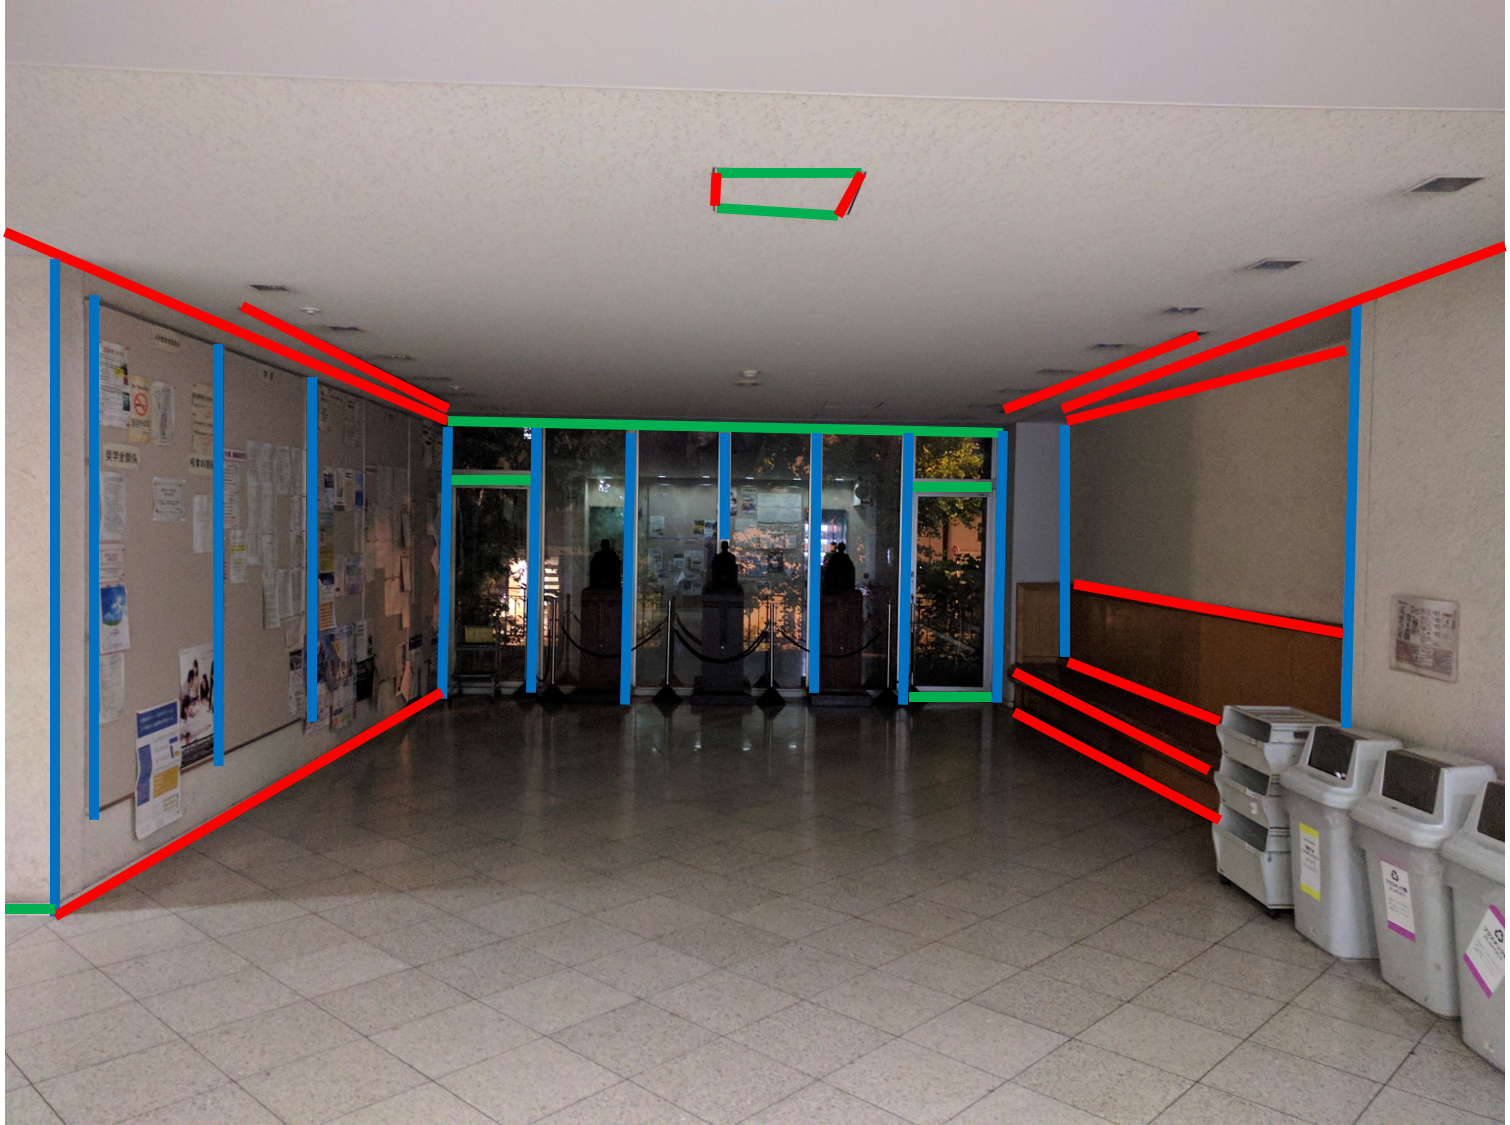
\includegraphics[width=0.7\columnwidth]{./chap2/fig/manhattan.png}
 \caption{屋内環境における互いに直交する3方向の直線の例}
 \label{fig:manhattan}
 \end{center}
\end{figure}

\newpage
\subsection{位置推定}

カメラの位置は,画像から生成した特徴量とラインマップの各位置から生成される特徴量を比較し,最も類似度の高い位置を探索することで推定することができる.
\\

Gotoらは,図\ref{fig:descriptor}に示すように,直線の長さに応じて重み付けされた,各直線が全天球カメラに投影されたときの大円の単位法線ベクトルの集合を特徴量として,Particle filter\mbox{\cite{Arulampalam2002}}\mbox{\cite{Arulampalam2004}}による全探索を行い位置を推定している\mbox{\cite{Goto2018}}.
しかし,Particle filterによる全探索は計算コストが高く,推定に時間がかかる.
\\

\begin{figure}[b]
 \begin{center}
 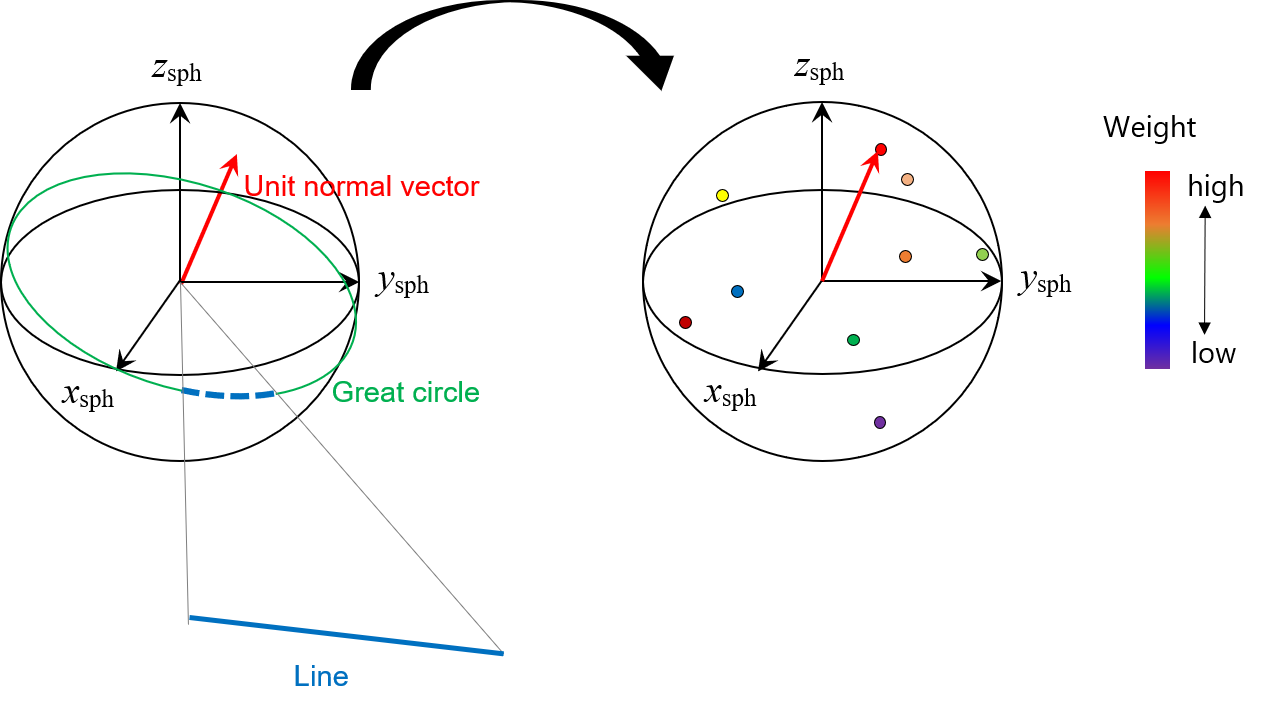
\includegraphics[width=0.9\columnwidth]{./chap2/fig/descriptor.png}
 \caption{[Goto 2018]における特徴量}
 \label{fig:descriptor}
 \end{center}
\end{figure}

本研究では,Levenberg-Marquardt法による非線形最適化を用いて探索することで高速に位置を推定する.
非線形最適化を用いる場合,局所解に陥る可能性があるという問題が生じる.
そこで,探索空間の次元を削減できる特徴量を新たに設計して用いることで,局所解に陥る可能性を低くする手法を提案する.


\clearpage
%==============================================================================
%おわりに
%==============================================================================
\section{おわりに}

本章では,本研究のアプローチについて述べた.

まず2.2節にて,本研究における問題設定について述べた.

2.3節にて,本手法の全体像について述べた.

2.4節にて,本手法のアプローチについて述べた.
2.4.1項にて,姿勢を推定するためのアプローチについて述べた.
2.4.2項にて,位置を推定するためのアプローチについて述べた.

次章では,姿勢推定の手法について詳しく説明する.


\clearpage
%%%%%%%%%%%%%%%%%%%%%%%%%%%%%%%%%%%%%%%%%%%%%%%%%%%%%%%%%%%%%%%%%%%%%%%%%%%%%%%
%%% Local Variables:
%%% mode: katex
%%% TeX-master: "../thesis"
%%% End: